\section{Another important celestial parameter: the obliquity}
\label{sec:6}
\begin{figure*}[b]
    \centering
    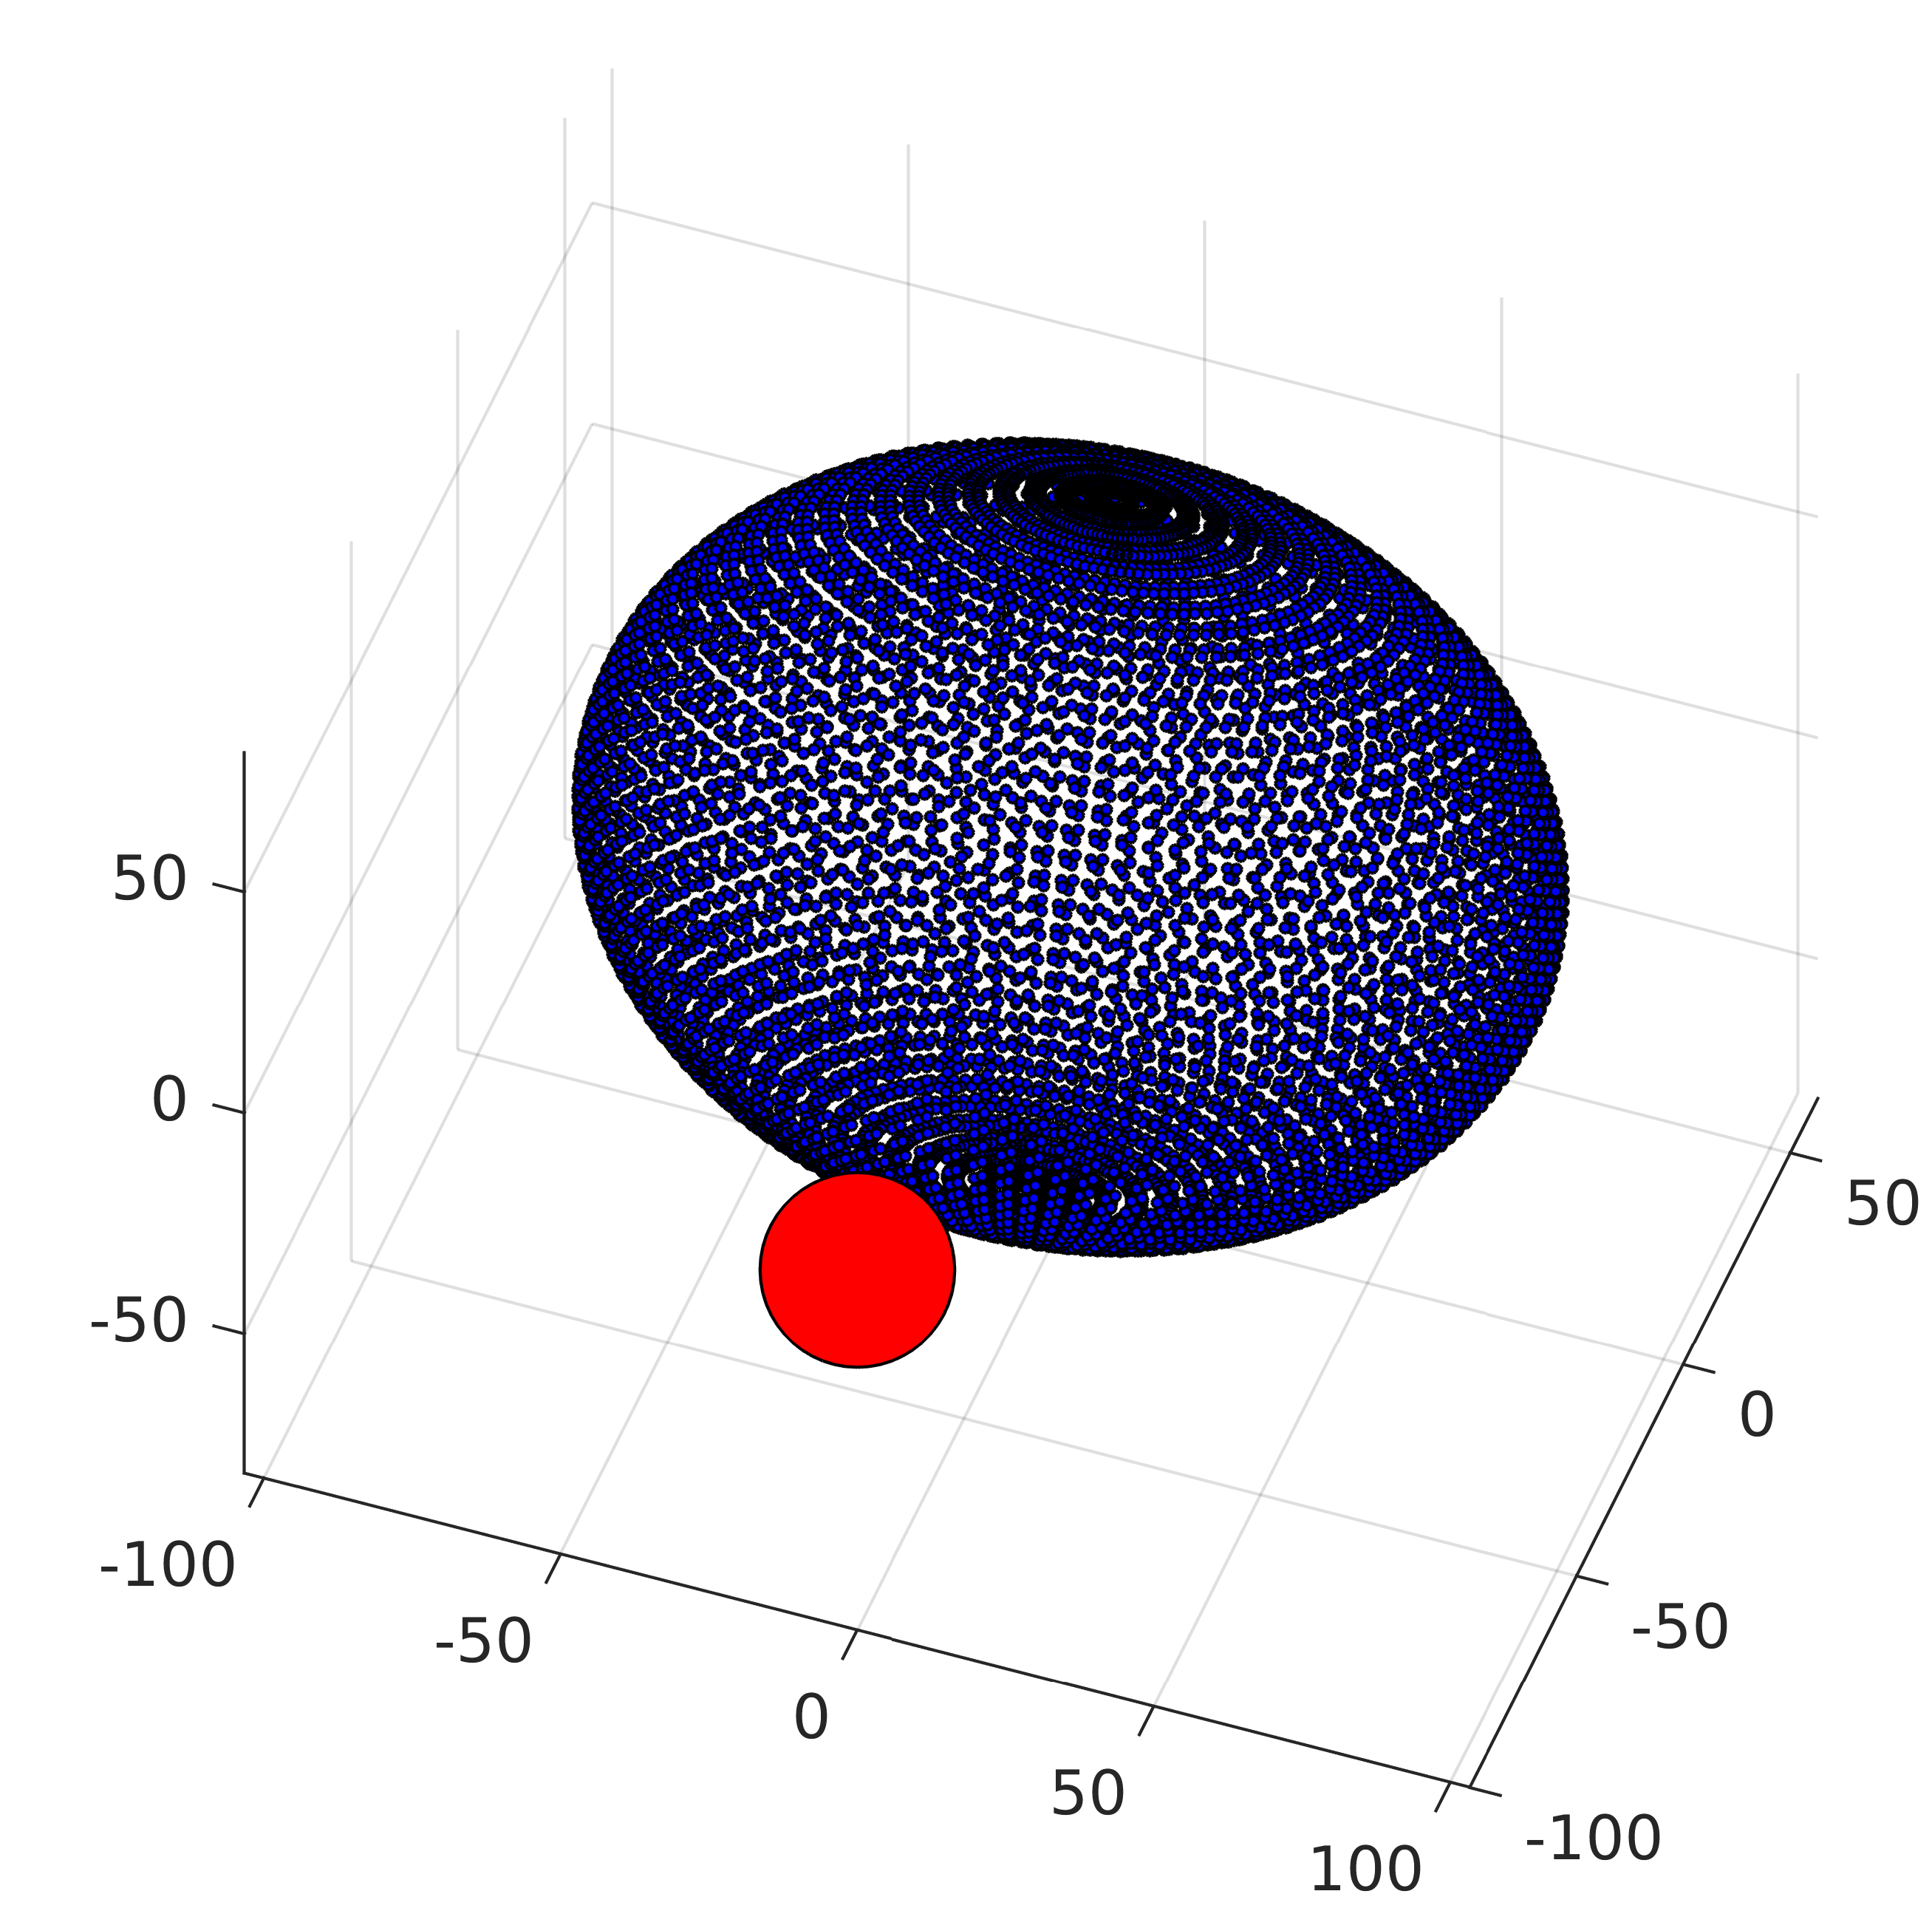
\includegraphics[width=0.33\linewidth]{rsc/obldemo1.png}
    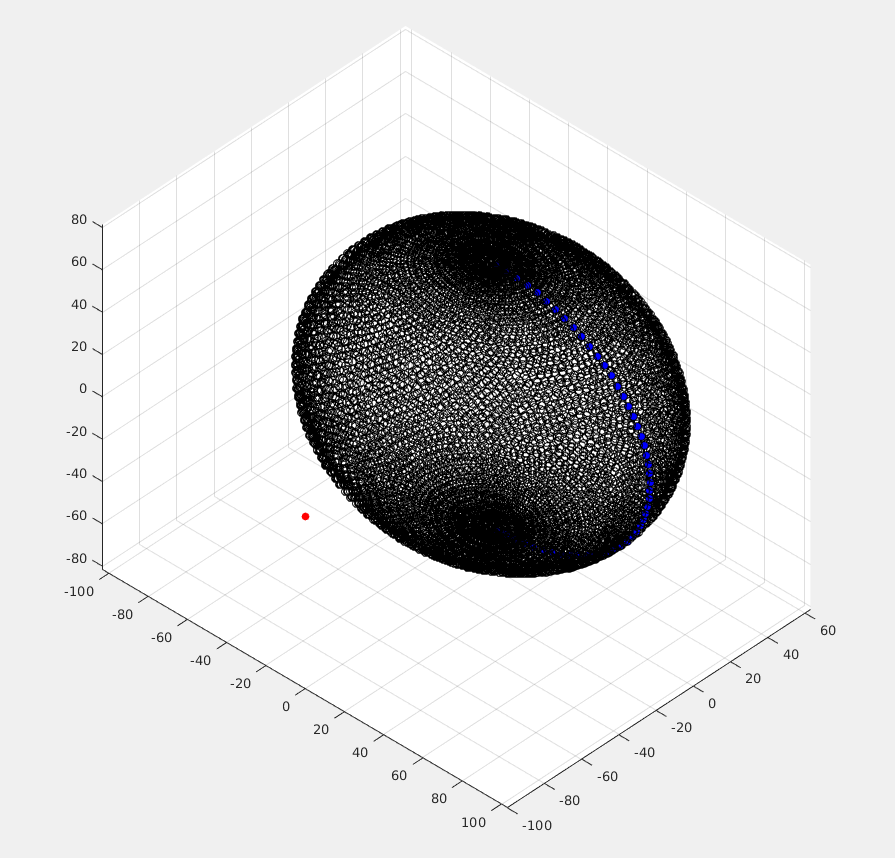
\includegraphics[width=0.33\linewidth]{rsc/obldemo2.png}
    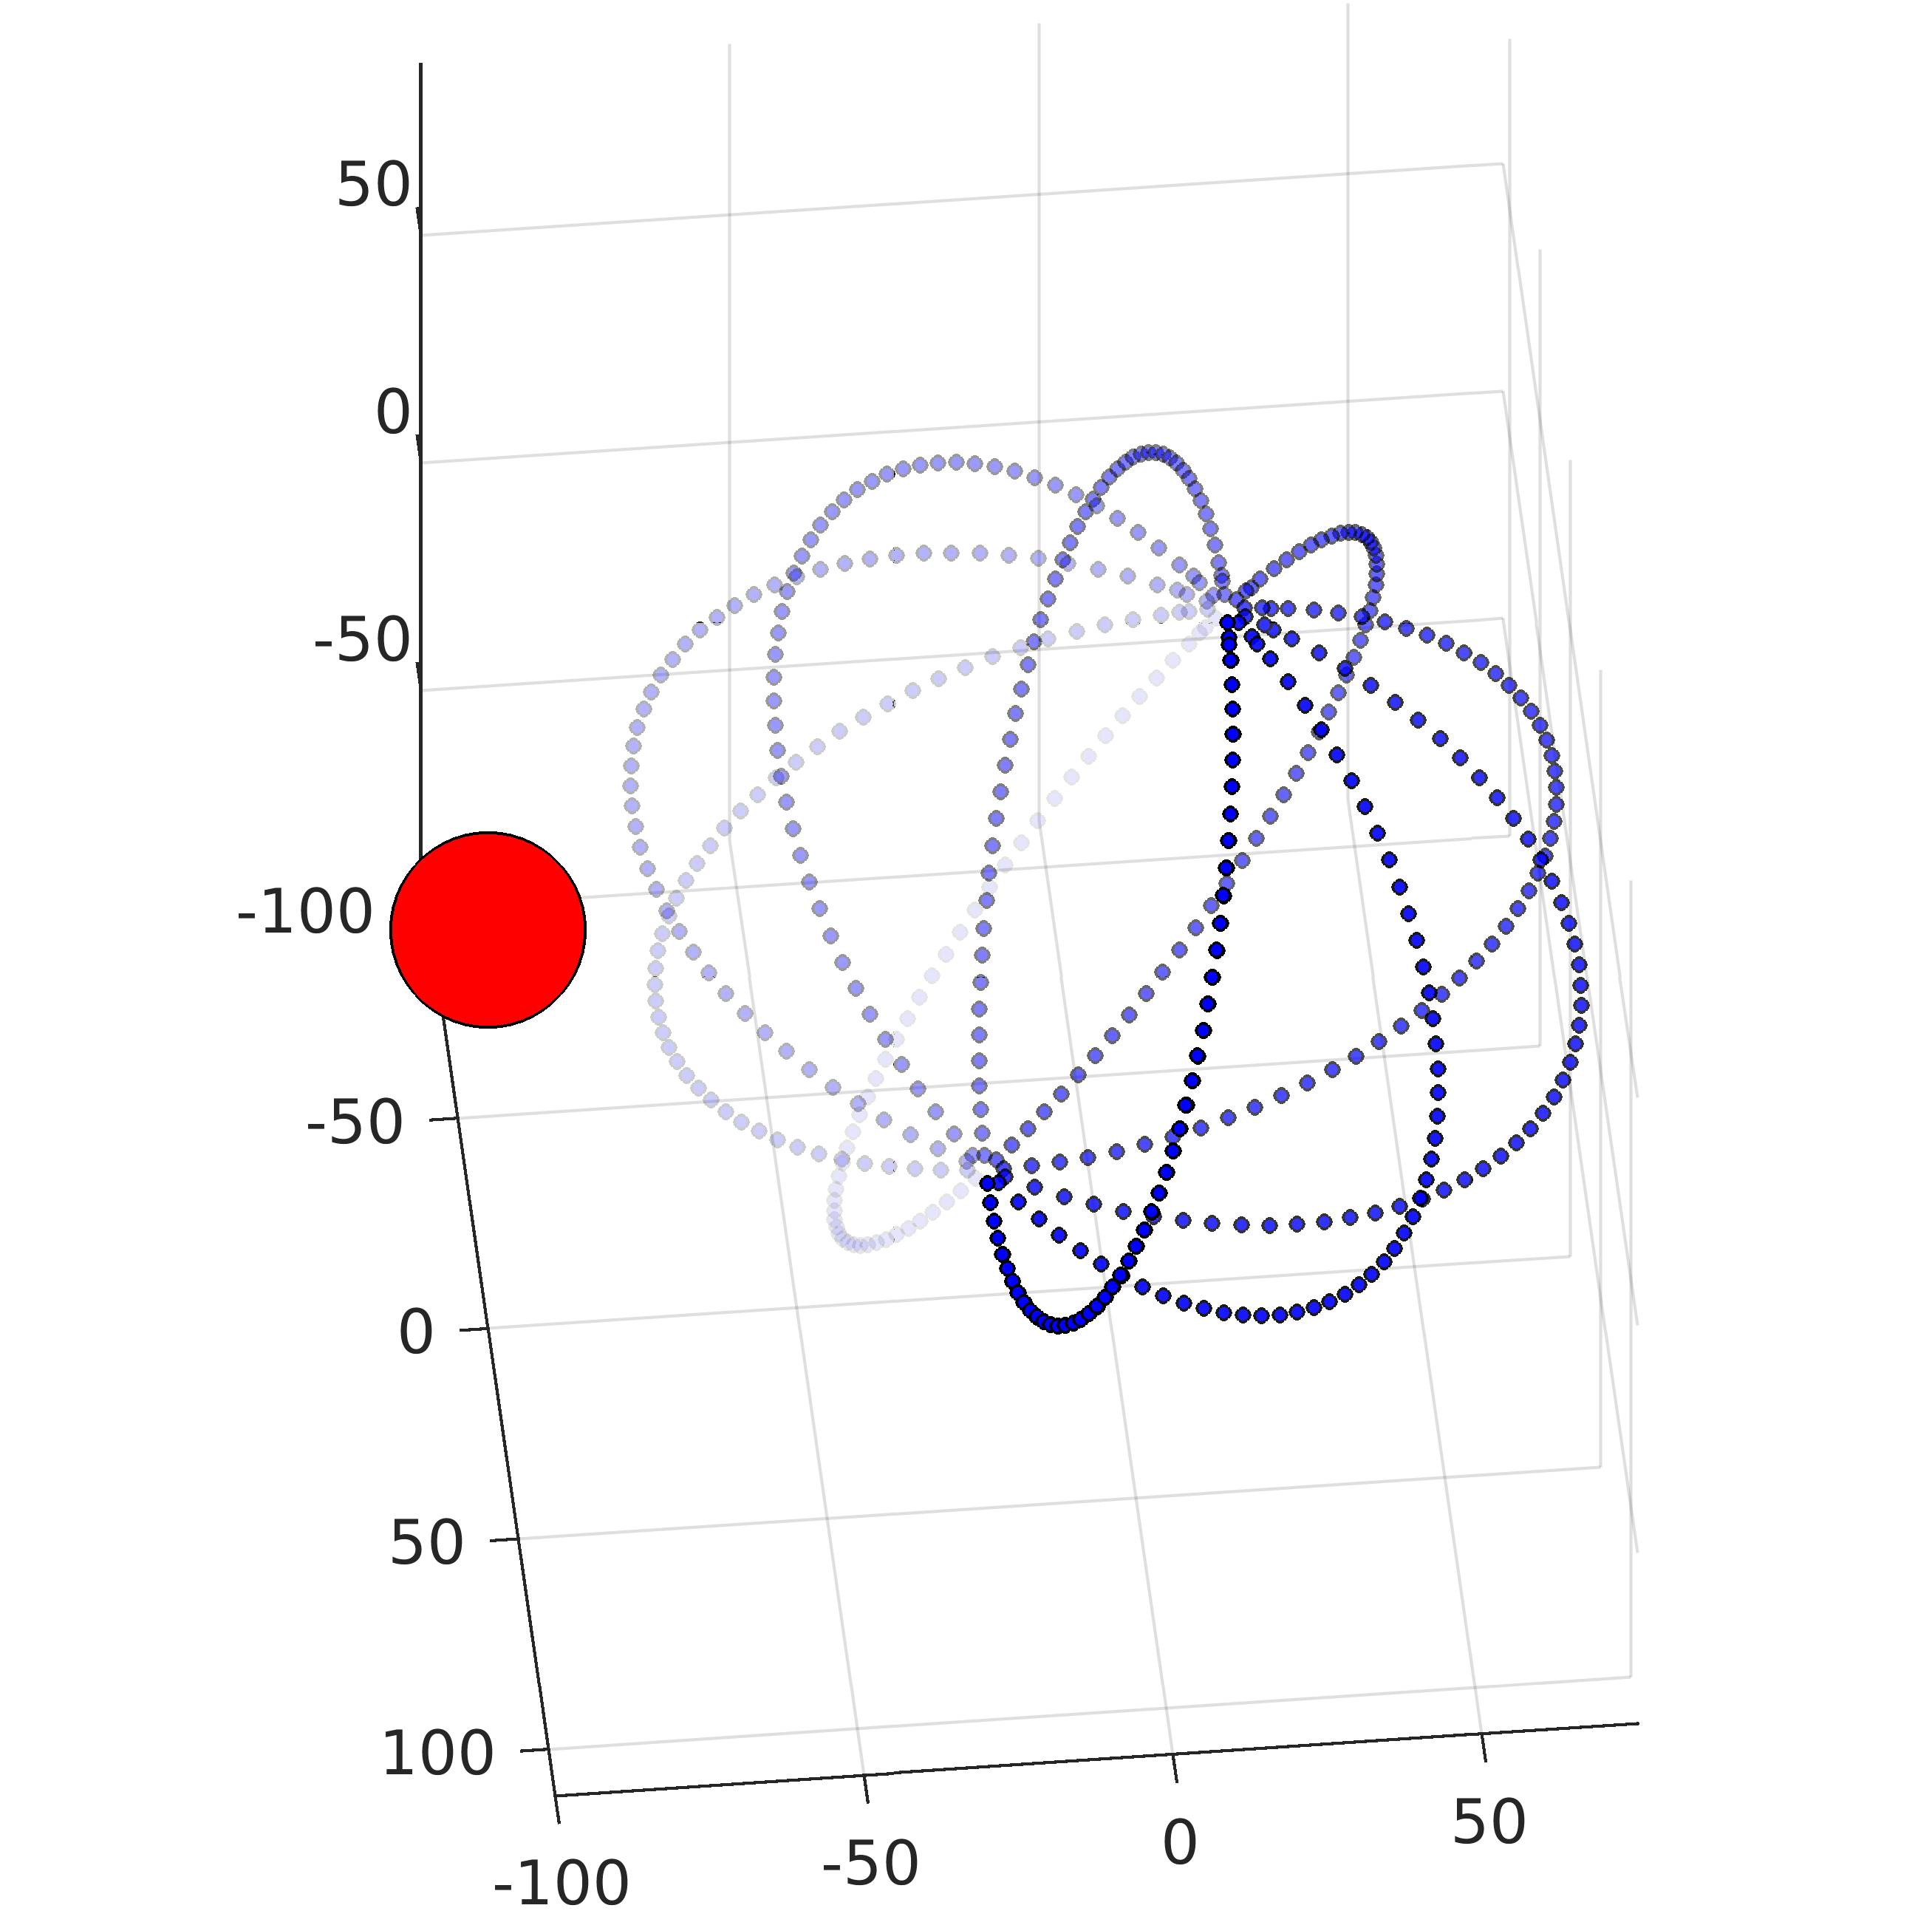
\includegraphics[width=0.33\linewidth]{rsc/obldemo3.png}
    \caption{Implementation of the obliquity for the daily surface temperature variation at longitude = 0 degrees on Didymos' secondary. The spin axis is given as 171 $\pm$ 9 degrees. Here, the extreme case of 162 degrees has been taken. The first figure is Didymoon's shape with obliquity and the direction of the Sun. On the second image we show only the meridian at longitude 0. The third pictures the rotation of the meridian during a day.}
\end{figure*}

This section describes the implementation of the obliquity and the explanation of the impact on the surface temperature. The obliquity is defined as the angle of tilt of the body's axis of rotation. Thus, it has an immediat impact on the repartition of temperature on the body as this figure describes: 
\begin{center}
    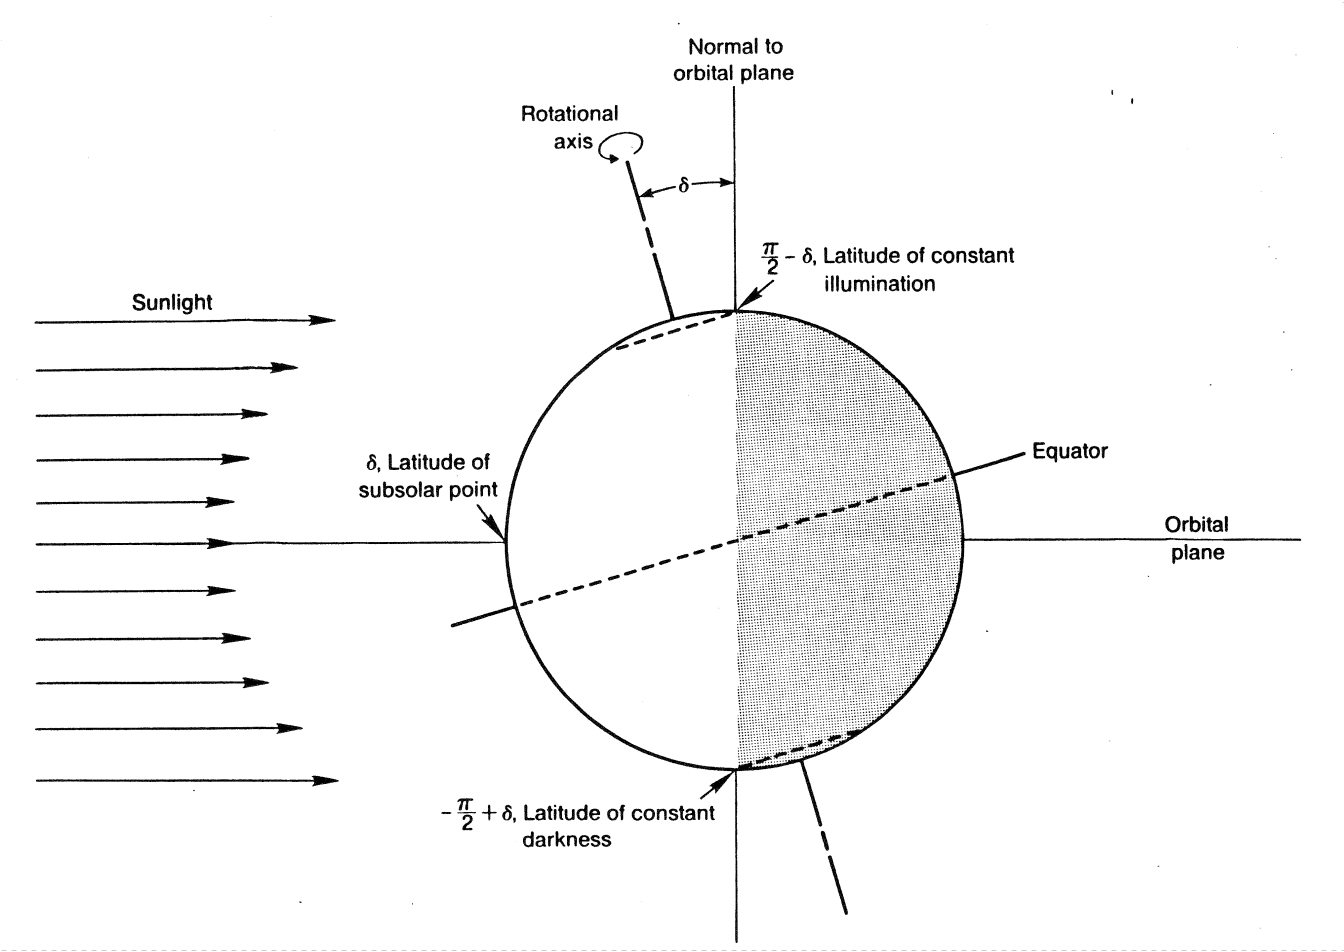
\includegraphics[width=\linewidth]{rsc/obliquity.png}
    \captionof{figure}{Representation of the obliquity with the orbital plane and the rotational axis}
\end{center}
From the obliquity results two observable events. First, the subsolar point is not anymore located on the equator but on a point tilted from the equator as the figure shows above. Secondly, depending on the position of the asteroid on its orbit - i.e. depending on the seasons, only one pole is not receiving direct heating from the Sun whereas without obliquity both poles are not receiving the heat.

Before running the simulations presented in the previous sections, we implement the axial tilt on the shape model.

Demonstration of the effects of the obliquity are performed for the temperature evolution of Didymos' secondary along a full day assuming an ellipsoidal shape.
\begin{figure*}[t]
    \centering
    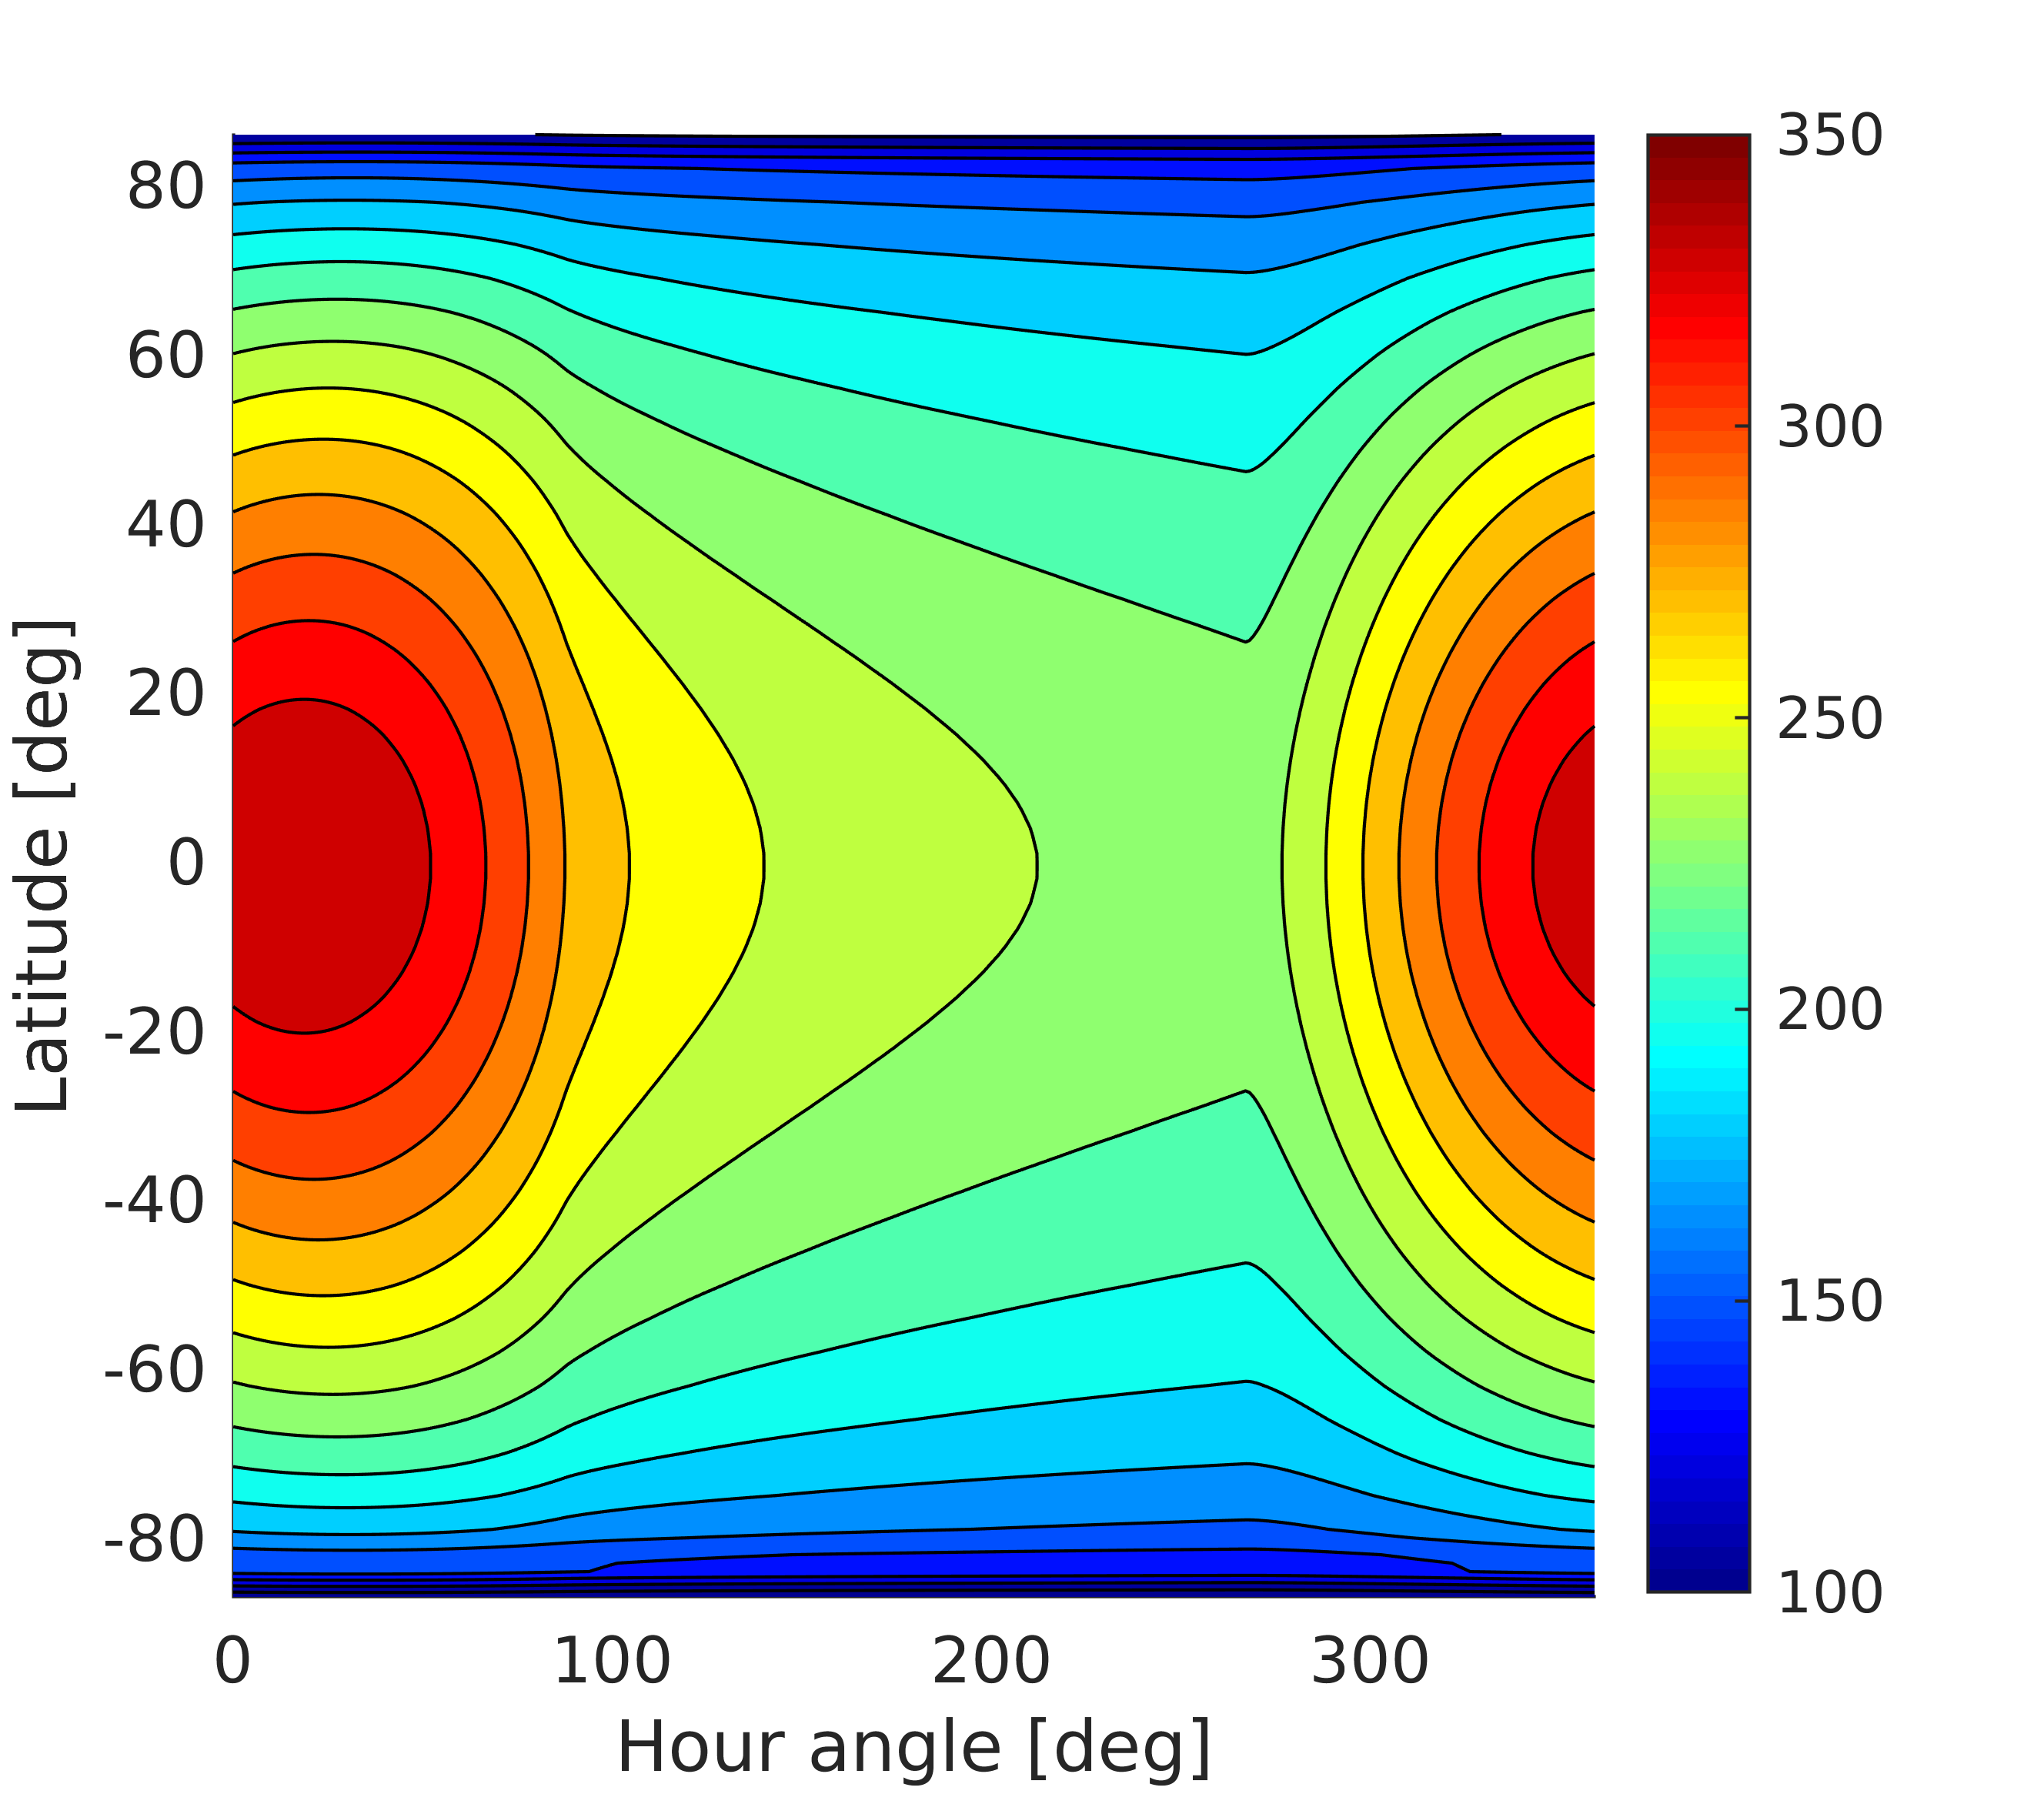
\includegraphics[width=0.45\linewidth]{rsc/hourangle_obl0.png}
    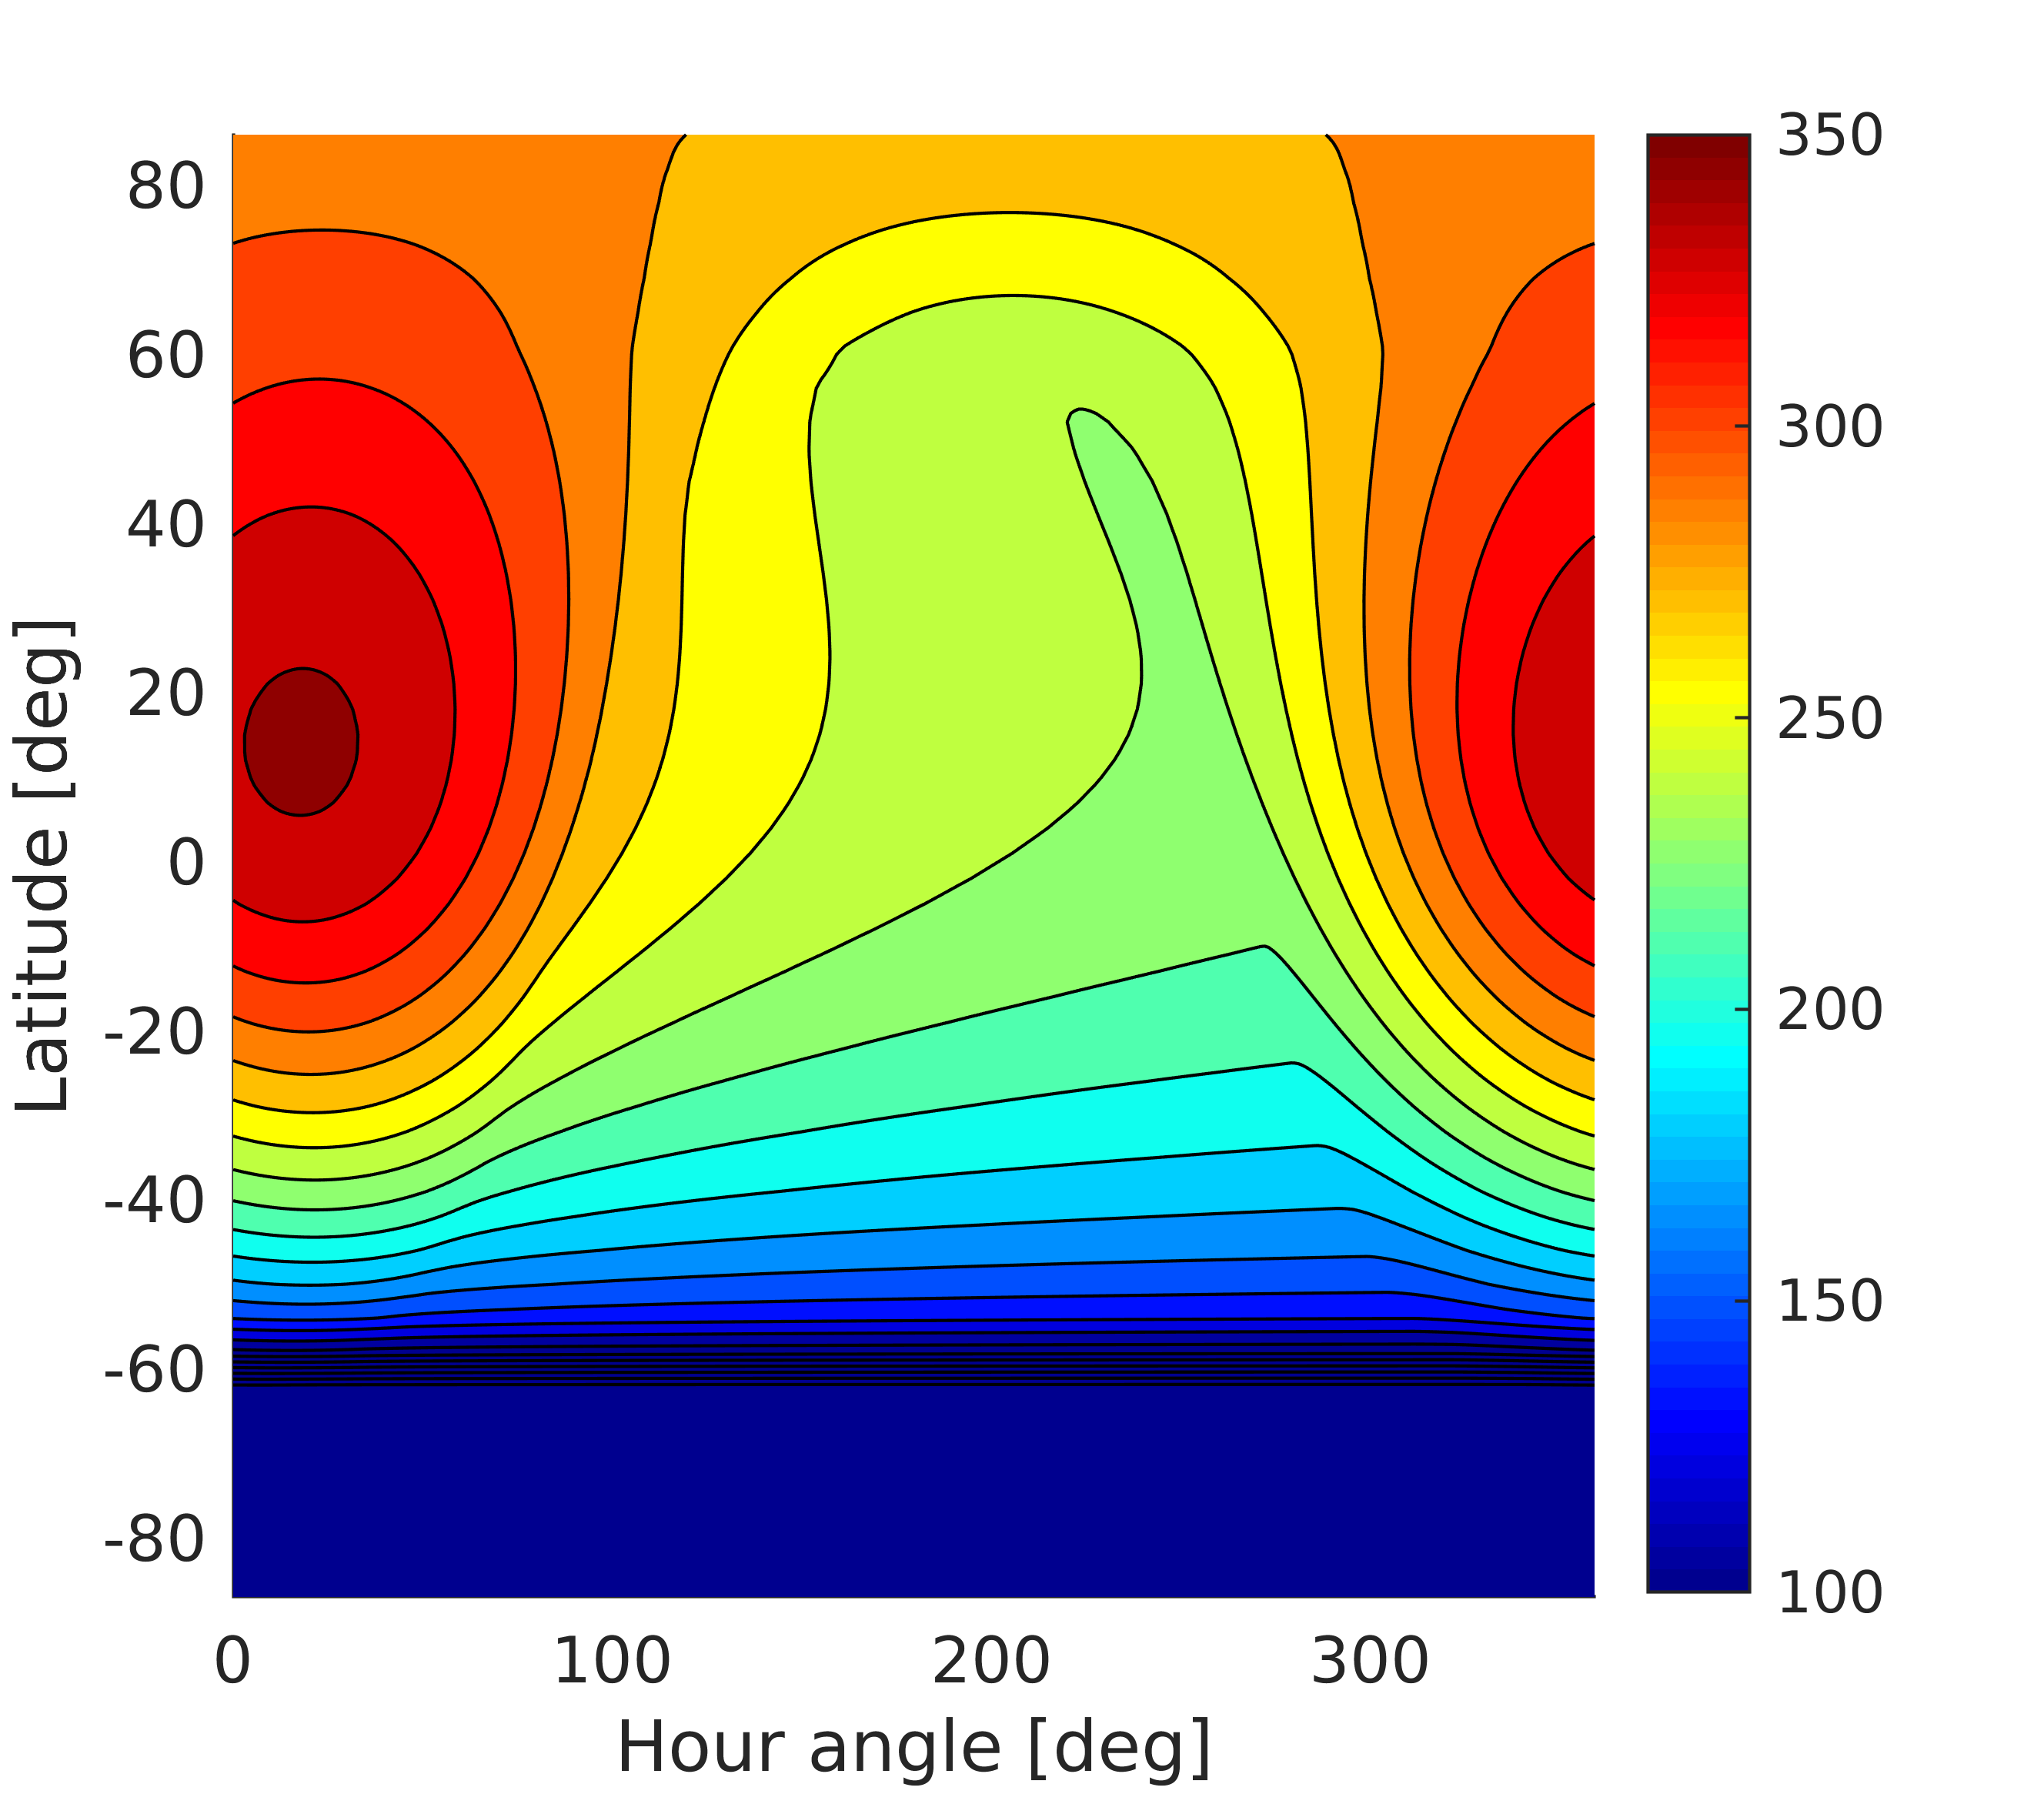
\includegraphics[width=0.45\linewidth]{rsc/hourangle_obl162.png}
    \caption{Contour maps of the daily surface temperature variation at longitude = 0 degree on Didymos' secondary for a thermal inertia of $\Gamma=500$ \si{Jm^{-2} K^{-1} s^{-1/2}}, an heliocentric distance of 1.0748 AU  and 162 degrees of obliquity.}
\end{figure*}
As expected, temperature peaks shift in latitudes depending on the obliquity and the south pole only is in the cold zone.
